%% Based on a TeXnicCenter-Template by Tino Weinkauf.
%%%%%%%%%%%%%%%%%%%%%%%%%%%%%%%%%%%%%%%%%%%%%%%%%%%%%%%%%%%%%

%%%%%%%%%%%%%%%%%%%%%%%%%%%%%%%%%%%%%%%%%%%%%%%%%%%%%%%%%%%%%
%% HEADER
%%%%%%%%%%%%%%%%%%%%%%%%%%%%%%%%%%%%%%%%%%%%%%%%%%%%%%%%%%%%%
\documentclass[letterpaper,twoside,10pt]{article}
% Alternative Options:
%	Paper Size: a4paper / a5paper / b5paper / letterpaper / legalpaper / executivepaper
% Duplex: oneside / twoside
% Base Font Size: 10pt / 11pt / 12pt


%% Language %%%%%%%%%%%%%%%%%%%%%%%%%%%%%%%%%%%%%%%%%%%%%%%%%
\usepackage[USenglish]{babel} %francais, polish, spanish, ...
\usepackage[T1]{fontenc}
%\usepackage[ansinew]{inputenc}

\usepackage{lmodern} %Type1-font for non-english texts and characters

\usepackage{amsmath}
\usepackage{braket}
\usepackage{floatrow}
\usepackage{subcaption}
\usepackage{natbib}
%\usepackage{appendix}


%% Packages for Graphics & Figures %%%%%%%%%%%%%%%%%%%%%%%%%%
\usepackage{graphicx} %%For loading graphic files
%\usepackage{subfig} %%Subfigures inside a figure
%\usepackage{pst-all} %%PSTricks - not useable with pdfLaTeX

%% Please note:
%% Images can be included using \includegraphics{Dateiname}
%% resp. using the dialog in the Insert menu.
%% 
%% The mode "LaTeX => PDF" allows the following formats:
%%   .jpg  .png  .pdf  .mps
%% 
%% The modes "LaTeX => DVI", "LaTeX => PS" und "LaTeX => PS => PDF"
%% allow the following formats:
%%   .eps  .ps  .bmp  .pict  .pntg


%% Math Packages %%%%%%%%%%%%%%%%%%%%%%%%%%%%%%%%%%%%%%%%%%%%
%\usepackage{amsmath}
%\usepackage{amsthm}
%\usepackage{amsfonts}


%% Line Spacing %%%%%%%%%%%%%%%%%%%%%%%%%%%%%%%%%%%%%%%%%%%%%
%\usepackage{setspace}
%\singlespacing        %% 1-spacing (default)
%\onehalfspacing       %% 1,5-spacing
%\doublespacing        %% 2-spacing

%% Other Packages %%%%%%%%%%%%%%%%%%%%%%%%%%%%%%%%%%%%%%%%%%%
\usepackage{a4wide} %%Smaller margins = more text per page.
%\usepackage{fancyhdr} %%Fancy headings
%\usepackage{longtable} %%For tables, that exceed one page


%%%%%%%%%%%%%%%%%%%%%%%%%%%%%%%%%%%%%%%%%%%%%%%%%%%%%%%%%%%%%
%% Remarks
%%%%%%%%%%%%%%%%%%%%%%%%%%%%%%%%%%%%%%%%%%%%%%%%%%%%%%%%%%%%%
%
% TODO:
% 1. Edit the used packages and their options (see above).
% 2. If you want, add a BibTeX-File to the project
%    (e.g., 'literature.bib').
% 3. Happy TeXing!
%
%%%%%%%%%%%%%%%%%%%%%%%%%%%%%%%%%%%%%%%%%%%%%%%%%%%%%%%%%%%%%

%%%%%%%%%%%%%%%%%%%%%%%%%%%%%%%%%%%%%%%%%%%%%%%%%%%%%%%%%%%%%
%% Options / Modifications
%%%%%%%%%%%%%%%%%%%%%%%%%%%%%%%%%%%%%%%%%%%%%%%%%%%%%%%%%%%%%

%\input{options} %You need a file 'options.tex' for this
%% ==> TeXnicCenter supplies some possible option files
%% ==> with its templates (File | New from Template...).



%%%%%%%%%%%%%%%%%%%%%%%%%%%%%%%%%%%%%%%%%%%%%%%%%%%%%%%%%%%%%
%% DOCUMENT
%%%%%%%%%%%%%%%%%%%%%%%%%%%%%%%%%%%%%%%%%%%%%%%%%%%%%%%%%%%%%
\begin{document}

\pagestyle{empty} %No headings for the first pages.


%% Title Page %%%%%%%%%%%%%%%%%%%%%%%%%%%%%%%%%%%%%%%%%%%%%%%
%% ==> Write your text here or include other files.

%% The simple version:
\title{Quantum Channel Capacities}
\author{John Rinehart}
%\date{} %%If commented, the current date is used.
\maketitle

%% The nice version:
%\input{titlepage} %%You need a file 'titlepage.tex' for this.
%% ==> TeXnicCenter supplies a possible titlepage file
%% ==> with its templates (File | New from Template...).


%% Inhaltsverzeichnis %%%%%%%%%%%%%%%%%%%%%%%%%%%%%%%%%%%%%%%
%\tableofcontents %Table of contents
%\cleardoublepage %The first chapter should start on an odd page.

\pagestyle{plain} %Now display headings: headings / fancy / ...



%% Chapters %%%%%%%%%%%%%%%%%%%%%%%%%%%%%%%%%%%%%%%%%%%%%%%%%
%% ==> Write your text here or include other files.

%\input{intro} %You need a file 'intro.tex' for this.


%%%%%%%%%%%%%%%%%%%%%%%%%%%%%%%%%%%%%%%%%%%%%%%%%%%%%%%%%%%%%
%% ==> Some hints are following:

\section{Introduction}
The formal study of ``information'' as a quantity is a relatively new undertaking. Claude Shannon's seminal work ``A Mathematical Theory of Communication'', published in 1948 quantified the power and limitations of a sender to reliably transfer information to the receiver. Several incredible results, including the ``noiseless coding theorem'' and the ``noisy-channel coding theorem'' were a direct result of this work. The fundamental nature and profound implications of this study have inspired countless other publications and have instigated new branches of mathematics and physics devoted to understanding the world in terms of information transfer. More recently, the revelation that low-energy physical systems adhere to the laws of the quantum mechanics has inspired the study of information according to the perspective of quantum states. The results of Shannon serving as a guide, this paper reformulates the definitions and results of classical information theory in the context of intrinsically richer and more complicated quantum systems.

\section{Classical Channel Capacities}

\subsection{Definitions and Elementary Results}
The first abstraction that must be made to allow for the study of information is to formalize how information is transferred. Information will be classified as any sequence of \textbf{symbols} (distinct entities) which are transferred between individuals utilizing a medium denoted as a \textbf{channel}. The \textbf{sender} transfers the information (symbols) at a given rate across the channel to the \textbf{receiver}. The sender and receiver can agree upon a \textbf{coding} scheme that allows the efficient use of the symbols. I.E. If the symbols to be transferred are Latin alphanumeric characters, it may be the case that the letter ``A'' and the numeral ``5'' are transmitted much less than ``F'' and ``1''; in which case, ``A'' and ``5'' are encoded using more binary digits than ``F'' and ``1'' so as to efficiently utilize the channel. If the channel has any sort of applied constraint, then there will be a limit on the number of signals that can be transmitted through it per unit time.

The prototypical example is that of the telegraphing channel. There, the transmission protocol used is that of the Morse code. The Morse code being the encoding scheme used, the channel would, typically, be a long length of conductive cabling. In this conductive cabling, susceptible to electromagnetic interference and random thermal agitations, the probability of an error occurring during transmission is non-zero. The occurrences of errors set a threshold on the amount of information that can be transferred across the cable. By transmitting a known sequence of symbols across the channel, the probability of an error occurring and the effective transmission rate of information can be determined. These assertions hold under the assumption that the noise behaves in a statistically consistent fashion (over many sequences) for all time (stationary) no matter what information is sent (ergodic).

Regarding the characterization of the sender: It may be the case that the sender is not transmitting much information. Such would be the case were a sender to transmit the date every few minutes. Considering the probability distribution of such a transmission, it would assign a high weighting to few symbols. Contrast this with the sender who transmits his/her life story by telegraph. In this case, the frequency of occurrence of all letters would be non-negligible given the finite transmission of the memoir. Thus, a way to quantify the amount of information being transferred is to consider the probability distribution over the available data set. The \textbf{Shannon entropy} does exactly this. Defined in the following way, the more uniform the probability distribution over the symbol set the larger the entropy: \begin{equation} H(\bar P) = -\sum_i p_i \log{p_i} \end{equation} $\bar P$ is defined as the set of the probabilities of transmitting all the available symbols $p_i$ : $\bar P = \{p_1,p_2,\cdots,p_n\}$. The base of the logarithms determines the fundamental unit of information. Using a base-2 logarithm the fundamental unit of information is the binary digit (bit). Using a base-10 logarithm the fundamental unit of information is the decimal digit. This can be expressed in the following way: Consider a set $ \bar A = \{X_1,X_2,\cdots,X_n\}$ with which is associated a set $ \bar P = \{p_1,p_2,\cdots,p_n\} $ such that each $X_i$ is associated with one and only one $p_i$ (injective) and such that $\sum_i p_i = 1$. $\bar A$ represents the alphabet and the elements of $\bar P$ yield the frequency of the elements of $\bar A$ occurring in the limit of an infinitely long sequence of symbols. 

An interesting case of a transmitted sequence $ S_i = \underbrace{X_i X_j \cdots X_k}_{\text{N symbols}} $ is one where N is assumed to be much larger that $|\bar A|$. Considering the limiting case where $S_i$ approaches an infinite length ($N \to\infty$) the distribution of symbols will approach $\bar P$ and the probability of a particular sequence, S', $P_{S'}$ occurring can be shown to be $P_{S'}=2^{-HN}$ and the number of such sequences can be shown to be $\# = 2^{HN}$ (See Appendix A).  Thus, fixing the alphabet and the N, the number of available transmittable sequences, $\#$, increases exponentially with the entropy of the source. For this reason, it is natural to talk about the source's entropy as being a direct measure of the amount of information producable by that source.

\subsection{Noiseless Channel Capacity}

Consider the case when the channel exhibits no noisy properties (referred to as the `ideal' channel). In this case, the medium can support as much information as is transmitted across it. Thus, the channel capacity (the amount of information able to be supported by the channel) is simply the rate of information transfer. If the transmitter encodes symbols into a certain number of bits (not necessarily the same for all symbols in the alphabet) then the transfer rate of symbols per second can be expressed in terms of bits per second (using an average in the case that symbols have unequal numbers of bits). 

\subsection{Noisy Channel Capacity}

However, the goal being to determine how much information can be transferred across a noisy channel, it becomes important to consider how the set of transmitted sequences, $\bar S_t$, is affected by the channel. Let $\bar S_r$ denote the set of all received sequences. The entropy of the transmitted sequences, $H_t$, is, in general, going to be different than the entropy of the received sequences, $H_r$. The rate of the channel can be defined by considering the amount of unambiguously received information. That is, the information transfer can be defined in terms of the amount of information intended to be sent by the transmitter and received by the receiver. Consider the case where a transmitted signal is corrupted by the channel so that the receiver is ignorant of some of the transmitted sequence. In this case, the information available to the receiver can be expressed as $H(\bar P_t) - H(\bar P_t | \bar P_r)$. A rigorous derivation of this expression is not given as it is a definition, not a fundamental result. However, the expression can be motivated by explaining the practical implications of the constituent terms. $H(\bar P_t)$ represents the amount of available information that \em could have \em been sent by the source (not having any knowledge as to what was received). $H(\bar P_t | \bar P_r)$ represents the amount of information that could have been sent by the source \em knowing what was received\em. In other words, the term $H(\bar P_t | \bar P_r)$ represents the amount of ignorance the receiver has regarding the amount of information that could have been sent. In this case, the transmitter can overcome the channel's loss by forcing a redundancy of $H(\bar P_t | \bar P_r)$ onto the encoded sequences. Thus, using a proper encoding scheme, the rate of transmitted errors can be reduced to be arbitrarily low. This is the amazing result. It may have been intuited that the amount of redundancy needed to transmit sequences across a noisy channel would have needed to continuously increase in order to achieve ever-lower frequencies of errors in transmission. However, the result is that, with a proper encoding scheme, a finite (bounded) amount of redundancy can be added to a sequence and still overcome the finite (bounded) noise of a channel. So, the capacity of the noisy channel is given by maximizing the prior expression over all the possible probability distributions of the input alphabet ($\bar P_i$). That is: \[C = \max_{\bar P_i}\Big(H(\bar P_i)-H(\bar P_i|\bar P_r)\Big) \]

Determining which set $\bar P_i$ accomplishes the least error rate is non-trivial. This is still an active area of research. However, it is nevertheless the case that proper encoding serves to limit the rate of errors to be arbitrarily small given an arbitrarily long transmitted sequence.
\section{Quantum Channel Capacities}


\subsection{Definitions and Elementary Results}
The approach that quantum information theorists have taken to quantum channels strongly resembles Shannon's approach to classical channels. However, quantum states, unlike classical states, have more degrees of freedom than the classical value obtained after measurement. Quantum states are endowed with the added properties of entanglement and superposition. That is, the effect of the channel on the states extends beyond the ability to toggle binary digits between 0 and 1. Rather, the channel can serve to destroy the phase information between basis states (channel decoherence) and/or corrode the entanglement of the states.

Now, in general, a pure state can be expressed as a linear combination of basis states. If that was all that was transmitted across the channel, then a description in terms of vectors (kets) would be sufficient. However, the fundamentally statistical nature of transmission begs a different representation for information. For this reason, the alphabet available to the quantum mechanical transmitter is spoken about and discussed using a set of density matrices. This allows for a more general and natural description of the information being communicated as well as lending itself to convenient descriptions of the various effects that the channel can have on the transmitted information.

The information being considered in its density formalism, it is natural to extend the form of the Shannon entropy (written in terms of probabilities) to a form appropriate for matrices. This quantum entropy must reduce to the classical entropy in the case where the alphabet of density states is formed using orthogonal states (essentially classical information, then). Hence, the Von Neumann entropy (the quantum mechanical analog of the classical Shannon entropy) is expressed as : $S(\rho)=-Tr(\rho\log(\rho))$. However, expressing $\rho$ in terms of its eigenbasis representation allows S to be calculated as follows: $S(\rho)=-\sum_i^d\lambda_i\log(\lambda_i)$, where $\lambda_i$ is the ith eigenvalue of $\rho$ and d is the dimensionality of $\rho$. Note that $\rho$ does not represent a particular alphabet symbol but, rather, $\rho$ represents the complete information about the symbols being sent and the probabilities of sending each of them. In other words, if $\rho_i$ is the ith alphabet symbol and $p_i$ is its probability of occurrence then $\rho = \sum_i p_i\rho_i$.

Now, consider the effect of noise on a state being transmitted across the channel. It is best to consider the effect of noise as being a map (in general, not unitary) : $\mathcal{E} : \rho \mapsto \rho'$. Now, if we want to represent the evolution of the channel \em and \em the state, then the evolution encompasses the entire universe so the evolution is unitary. This unitary evolution can be expressed as : $\mathcal{E}(\rho)=U\Big(\rho\otimes\ket{c_0}\bra{c_0}\Big)U^\dagger$, where $\ket{c_0}$ is the initial state of the environment. To obtain $\rho'$, all that is required is to trace out the channel: $\rho' = Tr_{c}{\mathcal{E}(\rho)}$. Expressing the trace in terms of a complete set of orthogonal channel states: $\mathcal{E}=\sum_i\bra{c_i}U\Big(\rho\otimes\ket{c_0}\bra{c_0}\Big)U^\dagger\ket{c_i}$. Here, U is a unitary operator that acts on the combined state of the channel and the prepared state. This can be expressed in a nice form by extracting everything but the transmitted state: $\sum_i\bra{c_i}U\ket{c_0}\rho\bra{c_0}U^\dagger\ket{c_i}$ and identifying the terms $\bra{c_i}U\ket{c_0}$ with the operators $E_i$ so that $\mathcal{E}=\sum_i E_i \rho E_i^\dagger$. This is known as the operator-sum representation of $\mathcal{E}$.

An interesting quality of quantum channel capacities is that they are a kind of superset of classical channel capacities. The classical channel can be modeled as a completely dephasing quantum channel. The properties of the quantum channel are also such that different capacities can be addressed when considering different operating conditions. For example, a  quantum channel that uses qubits to transfer classical information would, generally, have a capacity different than that of a quantum channel used to transfer the states of the qubits. In fact, interestingly enough, although it will not be shown here, the quantum capacities which have been solved have a smaller capacity than their classical counterpart. This may be justified by considering the sensitivity of the quantum states' to the noise. Superposition and entanglement are sensitive degrees of freedom which do not hold up under noisy conditions as well as does classical information (which has a higher threshold for error generation).

A quantum channel with feedback, with two-way communication, with a classical channel as a supplement are all entities which have different capacities. This makes determining the capacity of a quantum channel very difficult to do, in general. However, under certain conditions channel capacities have been determined and a discussion of these follow.

\subsection{General Channel Capacities}

\subsubsection{No-Entanglement-Single-Use Capacity}

Consider the channel where multiple channel uses are not allowed to entangle information between transmissions (only a single use of the channel is allowed per measurement). It can be imagined that the receiver can obtain a maximum amount of information, I, from the transmitted state. In analogy with the expression for the amount of information available to the receiver using a noisy classical channel, the amount of information available to the receiver using a noisy quantum channel is $I\le S(\rho)-\sum_ip_iS(\rho_i)$. The proof of this is given in Appendix B. 

Of course, similar to the noisy classical channel, the maximum amount of transferable information, is given by maximizing the amount of accessible information over all $\rho$'s. Thus, $C = \max_{\rho}(I)$. This, of course, is the capacity of the quantum channel in transmitting quantum information. This is not to say that this does not cover the case of transmitting classical information over the channel. For this case, all of the $\rho_i$'s are orthogonal and the Von Neumann entropy reduces to the Shannon entropy.

\subsubsection{No-Entanglement-N-Use Quantum Capacity}

Consider the case where entanglement is not allowed between uses of the quantum channel but the channel can be used an unbounded number of times before measurement. Such a use of the channel would result in transmitting a quantum state $\rho_p$ across the state n times so that the received state $\rho_r = \underbrace{\rho_p\otimes\rho_p\cdots\rho_p}_{n}$ (so-called block coding). In the limit of an infinite number of transmissions ($n\rightarrow\infty$), the capacity of the channel can be shown to saturate the bound given for the previous single-use channel capacity (see Appendix C): $C = \max_{\rho}\big(S(\rho)-\sum_ip_iS(\rho_i)\big)$. This result is the well-known Holevo-Westmoreland-Schumacher capacity (HSW capacity). For brevity, a proof of the HSW is not given here. The interested reader is directed to chapter 12 of reference 1 for more information.

\subsection{Specific Channel Capacities}
There are precious few channel capacities that have, until now, closed form expressions. A couple of these have already been given. In the context of these channels, different noise functions $\mathcal{E}$ can be studied. What follows is elementary analysis of a few types of noisy channels that are of interest to the theorist and the experimentalist.

\subsubsection{Bit Flip Channel}

The bit flip channel is a noisy channel that is defined as one in which the transmitted state $\rho_i$ is successfully received with probability p. However, with probability 1-p a transmitted qubit is replaced with a qubit where the roles of $\ket{0} \text{and} \ket{1}$ have been interchanged. In the case of a bit flip, a state $\Psi = a\ket{0}+b\ket{1} \mapsto \Psi'=b\ket{0}+a\ket{1}$. Thus, the density matrix transforms from $\ket{\Psi}\bra{\Psi}= \begin{pmatrix} |a|^2 & a^*b \\ ab^* & |b|^2 \end{pmatrix} \mapsto \ket{\Psi'}\bra{\Psi'}=\begin{pmatrix} |b|^2 & ab^* \\ a^*b & |a|^2 \end{pmatrix}$. In terms of the operator-sum form given earlier $\mathcal{E}(\rho) = (\sqrt p I)\rho (I\sqrt p)+\sqrt{1-p}X\rho X\sqrt{1-p} = p\rho + (1-p)X\rho X$.

The effect of this channel on an arbitrary qubit state can be described well in terms of the Bloch sphere representation. The following figure illustrates the effect of the bit flip channel on the Bloch sphere for different values of p. Graphically, the Bloch sphere is compressed along the Z and Y axes. The effect of the reduction along the Z-axis being that a measurement of the state in the Z-basis will return 0 and 1 with a probability approaching .5 (coin flip) as $p\rightarrow .5$.

\begin{figure}[H]%
\centering
	\begin{subfigure}{.3\textwidth}
		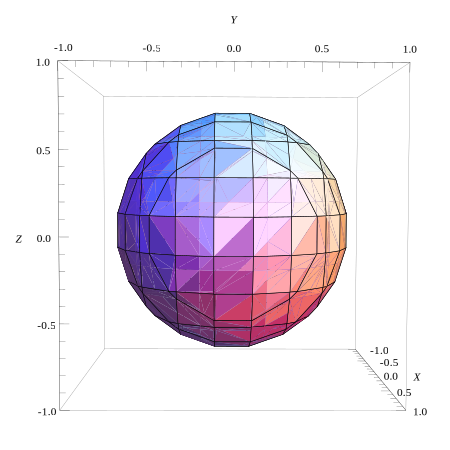
\includegraphics[width=\columnwidth,natwidth=300,natheight=300]{./BitFlip/BitFlipPoint1.pdf}%
		\caption{1-p = .1}%
	\end{subfigure}
	\begin{subfigure}{.3\textwidth}
		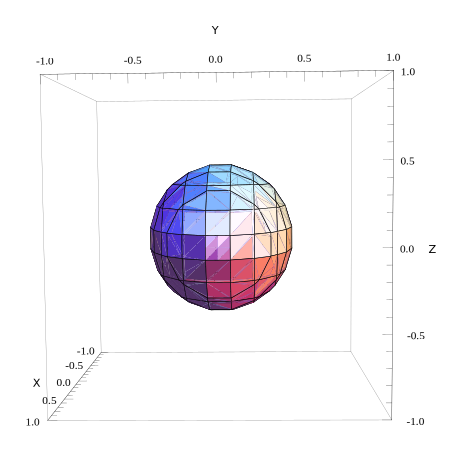
\includegraphics[width=\columnwidth,natwidth=300,natheight=300]{./BitFlip/BitFlipPoint25.pdf}%
		\caption{1-p =.25}%
	\end{subfigure}
	\begin{subfigure}{.3\textwidth}
		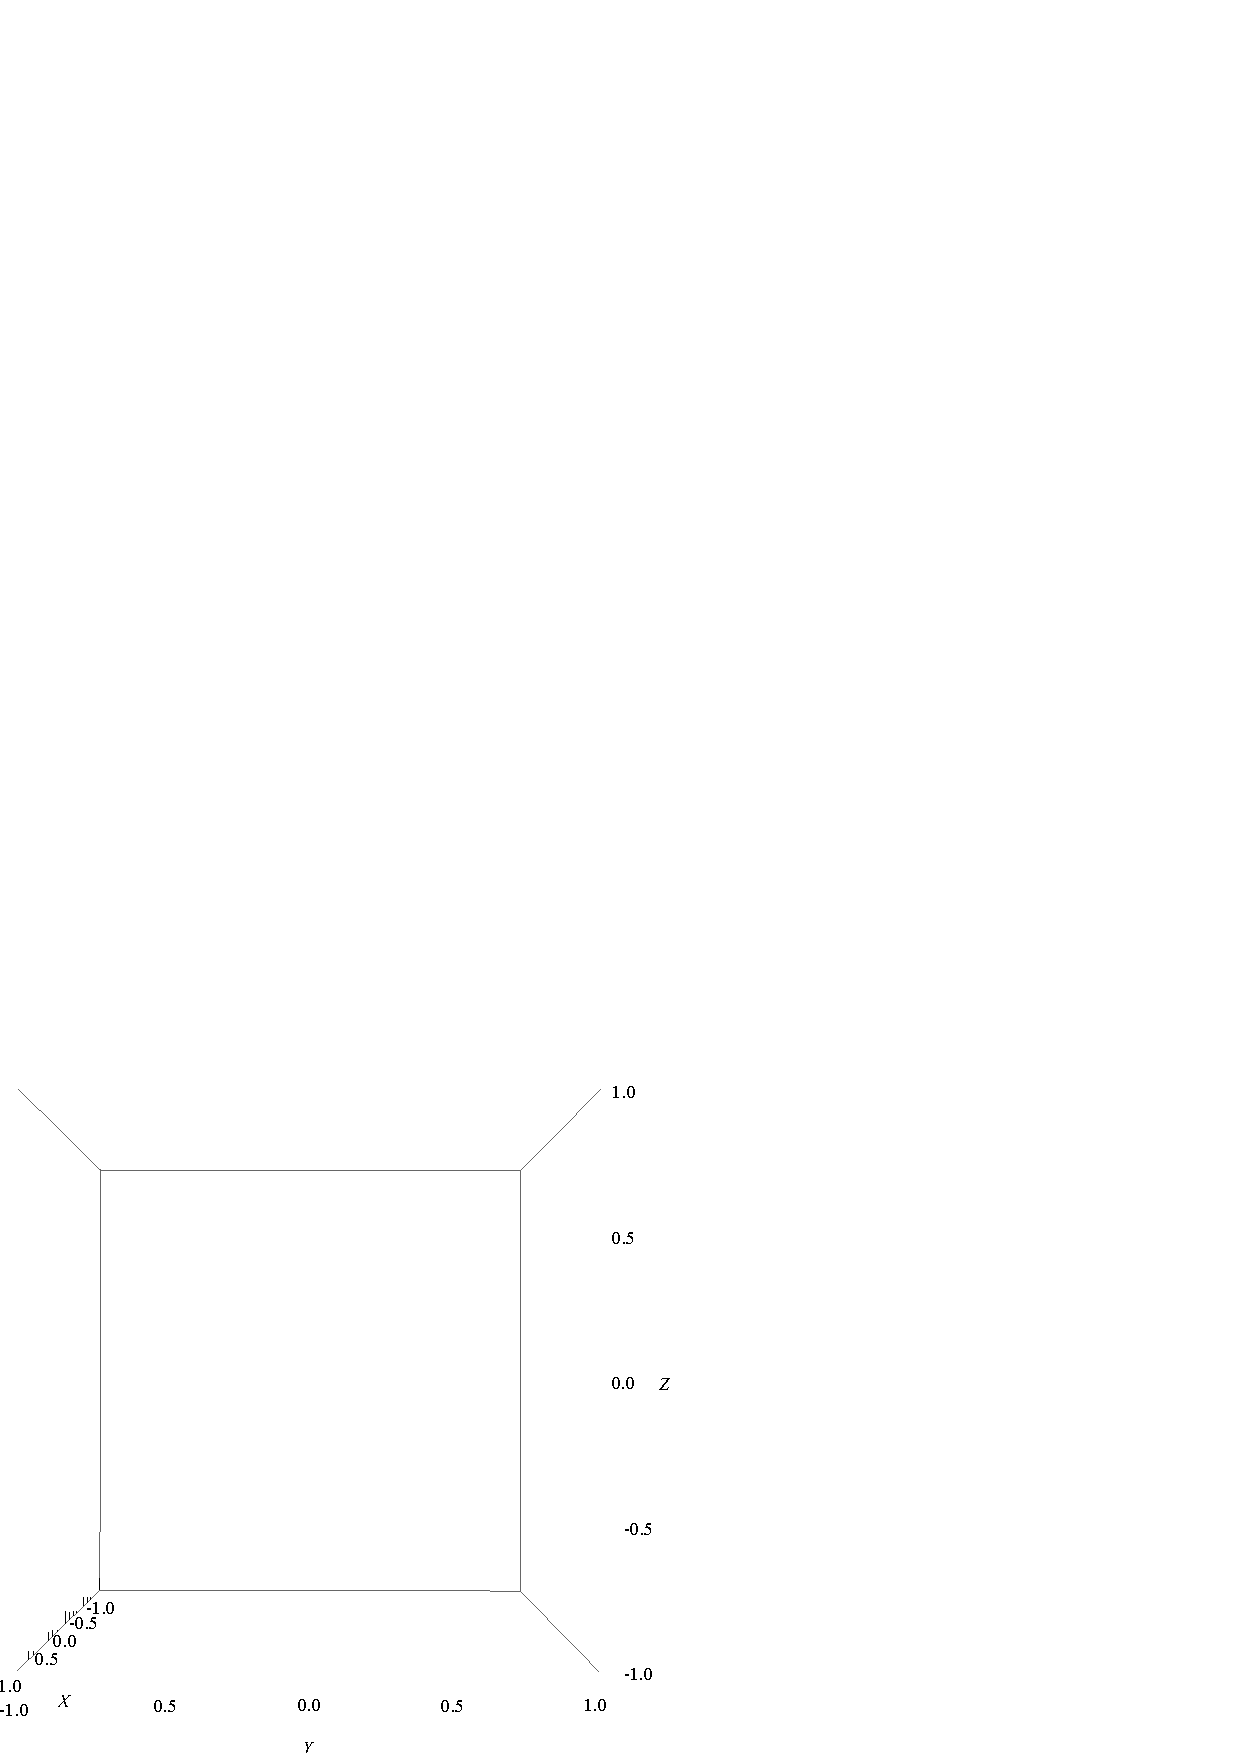
\includegraphics[width=\columnwidth,natwidth=300,natheight=300]{./BitFlip/BitFlipPoint4.pdf}%
		\caption{1-p =.4}%
	\end{subfigure}
	\caption{Effect of the Bit Flip Channel Using Varying Values of p.}
\end{figure}
	
\subsubsection{Phase Flip Channel}

The phase flip channel is a noisy channel that is defined as one in which the transmitted state $\rho_i$ is successfully received with probability p. However, with probability 1-p the state is replaced with a state whereby the sign of the phase on $\ket{1}$ has been switched. In the case of such a phase flip, a state $\Psi = a\ket{0}+b\ket{1} \mapsto \Psi'=a\ket{0}-b\ket{1}$. Thus, the density matrix transforms from $\ket{\Psi}\bra{\Psi}= \begin{pmatrix} |a|^2 & a^*b \\ ab^* & |b|^2 \end{pmatrix} \mapsto \ket{\Psi'}\bra{\Psi'}=\begin{pmatrix} |a|^2 & -ab^* \\ -a^*b & |b|^2 \end{pmatrix}$. In terms of the operator-sum form given earlier $\mathcal{E}(\rho) = (\sqrt p I)\rho (I\sqrt p)+\sqrt{1-p}Z\rho Z\sqrt{1-p} = p\rho + (1-p)Z\rho Z$. 

The following figure illustrates the effect of the phase flip channel on the Bloch sphere for different values of p. Similar to the bit flip channel, the Bloch sphere is compressed along the Y and X axes. The effect of the reduction along the non-Z axes being that a measurement of the state in the X-basis or Y-basis (to determine phase information of a state prepared in the Z-basis) will return 0 and 1 with a probability approaching .5 (coin flip) as $p\rightarrow .5$.

\begin{figure}[H]%
\centering
	\begin{subfigure}{.3\textwidth}
		\includegraphics[width=\columnwidth,natwidth=300,natheight=300]{./PhaseFlip/PhaseFlipPoint1.pdf}%
		\caption{1-p =.1}%
	\end{subfigure}
	\begin{subfigure}{.3\textwidth}
		\includegraphics[width=\columnwidth,natwidth=300,natheight=300]{./PhaseFlip/PhaseFlipPoint25.pdf}%
		\caption{1-p =.25}%
	\end{subfigure}
	\begin{subfigure}{.3\textwidth}
		\includegraphics[width=\columnwidth,natwidth=300,natheight=300]{./PhaseFlip/PhaseFlipPoint4.pdf}%
		\caption{1-p =.4}%
	\end{subfigure}
	\caption{Effect of the Phase Flip Channel Using Varying Values of p.}
\end{figure}
	
\subsubsection{Depolarizing Channel}

The depolarizing channel is a noisy channel that is defined as one in which the transmitted state $\rho_i$ is successfully received with probability p. However, with probability 1-p the state is replaced with a state that is a fully mixed (I/2). In this case, the density matrix transforms from $\ket{\Psi}\bra{\Psi}= \begin{pmatrix} |a|^2 & a^*b \\ ab^* & |b|^2 \end{pmatrix} \mapsto \ket{\Psi'}\bra{\Psi'}= \frac{1}{2}\begin{pmatrix} 1 & 0 \\ 0 & 1 \end{pmatrix}$. In terms of the operator-sum form given earlier $\mathcal{E}(\rho) = p\rho + \frac{(1-p)I}{2}$. 

The following figure illustrates the effect of the depolarizing channel on the Bloch sphere for different values of p. The Bloch sphere is compressed along all axes. The effect of this being to eliminate the probability of finding the received state in a pure state (regardless of the purity of the transmitted state).


\begin{figure}[H]%
\centering
	\begin{subfigure}{.3\textwidth}
		\includegraphics[width=\columnwidth,natwidth=550,natheight=550]{./Depolarizing/DepolarizingPoint1.pdf}%
		\caption{1-p =.1}%
	\end{subfigure}
	\begin{subfigure}{.3\textwidth}
		\includegraphics[width=\columnwidth,natwidth=550,natheight=550]{./Depolarizing/DepolarizingPoint25.pdf}%
		\caption{1-p =.25}%
	\end{subfigure}
	\begin{subfigure}{.3\textwidth}
		\includegraphics[width=\columnwidth,natwidth=550,natheight=550]{./Depolarizing/DepolarizingPoint4.pdf}%
		\caption{1-p =.4}%
	\end{subfigure}
	\caption{Effect of the Depolarizing Channel Using Varying Values of p.}
\end{figure}

\subsubsection{Amplitude Damping Channel}

The amplitude damping channel is a noisy channel that serves to remove energy from the transmitted state. This is a powerful model, since it can be used to simulate the effect of a real quantum system. In the laboratory, it is often the case that energy is dissipated into the bath (environment). It can be shown that the two quantum operators $E_0 = \begin{pmatrix}1 && 0 \\ 0 && \sqrt{1-p}\end{pmatrix}$ and $E_1=\begin{pmatrix}0 && \sqrt{p} \\ 0 && 0\end{pmatrix}$ can be used to form the noise map $\mathcal{E}=E_0\rho E_0^\dagger+E_1\rho E_1^\dagger$. 

The following figure illustrates the effect of the amplitude damping channel on the Bloch sphere for different values of p. Note that for increasing value of p, the Bloch sphere is compressed toward the $\ket{0}$ state in the Z-basis. This corresponds to the state losing energy when considering the $\ket{0}$ state to be the ground state of the qubit. Thus, p can be interpreted as the the probability of losing energy to the channel.

\begin{figure}[H]%
\centering
	\begin{subfigure}{.3\textwidth}
		\includegraphics[width=\columnwidth,natwidth=600,natheight=600]{./AmplitudeDamping/ADPoint2.pdf}%
		\caption{p =.1}%
	\end{subfigure}
	\begin{subfigure}{.3\textwidth}
		\includegraphics[width=\columnwidth,natwidth=600,natheight=600]{./AmplitudeDamping/ADPoint5.pdf}%
		\caption{p =.25}%
	\end{subfigure}
	\begin{subfigure}{.3\textwidth}
		\includegraphics[width=\columnwidth,natwidth=600,natheight=600]{./AmplitudeDamping/ADPoint8.pdf}%
		\caption{p =.4}%
	\end{subfigure}
	\caption{Effect of the Depolarizing Channel Using Varying Values of p.}
\end{figure}

%% <== End of hints
%%%%%%%%%%%%%%%%%%%%%%%%%%%%%%%%%%%%%%%%%%%%%%%%%%%%%%%%%%%%%



%%%%%%%%%%%%%%%%%%%%%%%%%%%%%%%%%%%%%%%%%%%%%%%%%%%%%%%%%%%%%
%% BIBLIOGRAPHY AND OTHER LISTS
%%%%%%%%%%%%%%%%%%%%%%%%%%%%%%%%%%%%%%%%%%%%%%%%%%%%%%%%%%%%%
%% A small distance to the other stuff in the table of contents (toc)
\addtocontents{toc}{\protect\vspace*{\baselineskip}}


%% The Bibliography
%% ==> You need a file 'literature.bib' for this.
%% ==> You need to run BibTeX for this (Project | Properties... | Uses BibTeX)
%\addcontentsline{toc}{chapter}{Bibliography} %'Bibliography' into toc
\nocite{*} %Even non-cited BibTeX-Entries will be shown.
\bibliographystyle{plain} %Style of Bibliography: plain / apalike / amsalpha / ...
\bibliography{references} %You need a file 'literature.bib' for this.

%%% The List of Figures
%\clearpage
%\addcontentsline{toc}{chapter}{List of Figures}
%\listoffigures
%
%%% The List of Tables
%\clearpage
%\addcontentsline{toc}{chapter}{List of Tables}
%\listoftables


%%%%%%%%%%%%%%%%%%%%%%%%%%%%%%%%%%%%%%%%%%%%%%%%%%%%%%%%%%%%%
%% APPENDICES
%%%%%%%%%%%%%%%%%%%%%%%%%%%%%%%%%%%%%%%%%%%%%%%%%%%%%%%%%%%%%

\appendix
\renewcommand\thesection{Appendix \Alph{section}}
\section{}


 \[ \#(S_i) = \frac{N!}{(n_1)!(n_2)!\cdots(n_n)!} \] 

where $n_i$ indicates the number of $X_i$'s that have occurred in the sequence from the alphabet. Taking the logarithm of both sides and rearranging yields: 

\[\log(\#) = \log(N!)- \log(n_1!)-\log(n_2!)-\cdots-\log(n_n!) \]

Assuming N is very large (and, so all the $n_i$'s are correspondingly large) it is appropriate to write $N!\approx N\log(N)$, using Stirling's formula, so that $\log(\#)$ becomes 

\[\log(\#) = N\log(N)-n_1\log(n_1)-n_2\log(n_2)\cdots-n_n\log(n_n) \]

Realizing that the number of $X_i$'s that occur in a sequence ($n_i$) is proportional to the probability that $X_i$ occurs yields,

\[\log(\#) = N\log(N)-Np_1\log(Np_1)-Np_2\log(Np_2)-\cdots-Np_n\log(Np_n)\]

which reduces nicely to

\[\log(\#)=N\log(N)-N\log(N)\sum_ip_i-N\sum_ip_i\log(p_i) = NH \]

since $\sum_ip_i = 1$ and $\sum_ip_i\log p_i = -H$. Thus the number of such sequence goes as $\# = 2^{NH}$ (using a bit as the fundamental unit of information).

Now, consider the probability of a particular sequence $s$ to occur, $P_s$. Assuming the probability of transmitting individual symbols is independent, the probability of such a sequence can be expressed as follows: $P_s = p_1^{Np_1}p_2^{Np_2}\cdots p_n^{Np_n}$. Taking the logarithm of both sides 
\[
\log(P_s)=Np_1\log(p_1)+Np_2\log(p_2)+\cdots+Np_n\log(p_n))
\]
\[
= N(p_1\log(p_1)+p_2\log(p_2)+\cdots+p_n\log(p_n) = -NH
\]
Thus, $P_s = 2^{-NH}$.

This agrees well with the number of sequences occurring as $2^{NH}$ since the total probability of all these sequences occurring should be $\approx 1$.

%% ==> Write your text here or include other files.

%\input{FileName} %You need a file 'FileName.tex' for this.

\section{Demonstration of Holevo's Bound}

This derivation has been replicated using Nielsen and Chuang's ``Quantum Information and Quantum Computation'' (reference 1). Consider three spaces: A,B and P. Allow Alice to prepare a state in the space A. Allow a receiver Bob to receive the state in the space B. P is an intermediate space to allow the transfer of the prepared state (A) to Bob (B). The goal will be to compare the combined (mutual) entropy of A and P before the state transfer to the mutual information shared between A and B after the state transfer. Allow the initial state, prepared by Alice to be $\rho=\sum_xp_x\ket{x}\bra{x}$. Thus, assuming Bob's initial state is $\ket{0}\bra{0}$ the combined state between A, B and P can be expressed as : $\rho_{sys}= \rho_A\otimes\rho_P\otimes\rho_B=\rho_{sys}=\sum_x p_x\ket{x}\bra{x}\otimes\rho_x \otimes \ket{0}\bra{0}$.

\subsection{Entropy Prior to State Transfer}
Now, consider the quantity $S(\rho_A:\rho_B)$. Since B provides no extra information to the system (Alice is assumed to be the source of all information), then $S(\rho_A:\rho_P)=S(\rho_A:\rho_P,\rho_B)$ where $S(\rho_A:\rho_P,\rho_B)$ is the mutual entropy shared between A and the combined systems P and B. Now, it can be shown that the entropy of the system is not increased after a general quantum measurement. Thus, once Bob has measured the state Alice has sent him, the entropy of the system is either the same or smaller. 

Use primes to denote the post-measurement spaces A',B',P' - the spaces have the same dimensionality before and after measurement, but the information contained within them is different. $S(\rho_A:\rho_P,\rho_B)\ge S(\rho_{A'}:\rho_{P'},\rho_{B'})$ for aforementioned reasons. If we consider tracing out the state P' we realize the entropy must either stay the same or decrease (it can not increase). A natural way to express this is by saying that removing a space of interest can not increase the total entropy/amount of information. Thus, $S(\rho_A:\rho_P)\ge S(\rho_{A'}:\rho_{B'})$.

Consider $S(\rho_A:\rho_P) = S(\rho_A)+S(\rho_P)-S(\rho_A,\rho_P) $ , the mutual entropy between space A and P (the expression being a fundamental result of considering joint and mutual entropies). Since the state in space A has been expressed in its diagonal form, $S(\rho_A)=H(\bar {P_x})$ (the Shannon entropy over Alice's probability distribution). The entropy of P is simply the entropy of the prepared state $\rho$: $S(\rho_P)=S(\rho)$. $S(\rho_A,\rho_P)=H(\bar {P_X})+\sum_i p_i S(\rho_i)$ due to the uncorrelated and orthogonal nature of the spaces A and P (for more information, the interested reader is directed to chapter 11 of reference 1). Thus, $S(\rho_A:\rho_P)=S(\rho)-\sum_i p_iS(\rho_i)$.

\subsection{Entropy After State Transfer}
To conclude this proof we need to consider the mutual information between Alice and Bob after the state has been transferred. The way in which information is to be transferred to Bob is to use a generalized quantum operation that measures the state in system P and transfers that to Bob's system. This transfer can be expressed in the following way: $\mathcal{E}: \alpha \otimes \ket{0}\bra{0} \mapsto \sum_b \sqrt{E_b}\alpha\sqrt{E_b}\otimes\ket{b}\bra{b}$ where b is an orthogonal basis for Bob's space and $E_y$ are the generalized quantum operators. The state of the entire system post-measurement is then : $\sum_y\sum_xp_x\ket{x}\bra{x}\otimes\sqrt{E_b}\rho_x\sqrt{E_b}\otimes\ket{b}\bra{b}$. Tracing out the unwanted P' system : $\rho_{A',B'} =  \sum_y\sum_x p_x\ket{x}\bra{x} \cdot Tr(\sqrt{E_b}\rho_x\sqrt{E_b})\cdot\ket{b}\bra{b}$. Then, making the realization that $p_x Tr(\sqrt{E_b}\rho_x\sqrt{E_b})$ is the same thing as the joint probability of x and b, $p(x,b)$, the state is rewritten : $\rho_{A',B'} =  \sum_y\sum_x p(x,y) \ket{x}\bra{x}\otimes\ket{b}\bra{b}$. Written this way it can be seen that the entropy between A' and B' (joint and mutual) are, $S(\rho_{A'},\rho_{B'}) = H(\bar{P_x},\bar{P_b})~\text{and}~S(\rho_{A'}:\rho_{B'})=H(\bar{P_x}:\bar{P_b})$.

Finally, realizing that from earlier $S(\rho_A:\rho_P)\ge S(\rho_{A'}:\rho_{B})$ the result follows : $S(\rho)-\sum_ip_iS(\rho_i) \ge H(\bar{P_x}:\bar{P_b})$. This is a pretty incredible statement. The results declares directly that there is a maximum amount of information about the state $\rho$ that we can determine with a single measurement. This may be obvious to the introductory student of the quantum mechanics. However, more impressively, this statement gives you the \em amount of information \em that you can obtain, at most, when having received a density state $\rho_x$ with some probability $p_x$.  As an aside, the quantity on the side of the inequality involving quantum Von Neumann entropies is referred to as the Holevo information. It is a term which appears when determining the capacity of a quantum channel to support information transfer.


\end{document}
